\section{Results}

\subsection{Motor Friction Estimation}
Pendulum angle \(\theta\) was sampled with a sampling rate of 60Hz. \(\dot{\theta}\) and \(\ddot{\theta}\) were derived from \(\theta\) using numerical differentiation. The viscous damping coefficient \( b \) was found to be \( 0.001 \) Nm/rad/s for the hip motors (A20 etc) and \( 0.0001 \) Nm/rad/s for the knee motors (A14 etc). Figures \ref{fig:results:motor_friction_estimation:linear_regression_knee_motor} and \ref{fig:results:motor_friction_estimation:linear_regression_hip_motor} show the the predicted \(\dot{\theta}\) from the physical models of the pendulum using the estimated viscous damping coefficients, versus the derived \(\dot{\theta}\).

\begin{figure}[h]
    \centering
    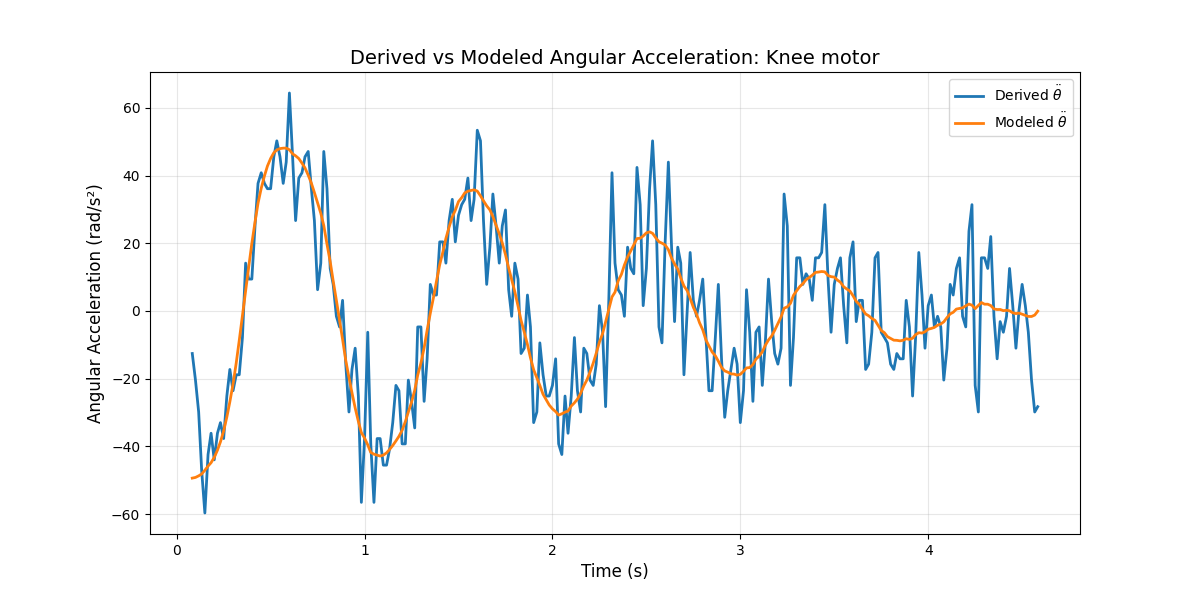
\includegraphics[width=0.8\textwidth]{Images/results/friction_est_knee_motor.png}
    \caption{Linear regression fit of the pendulum data for the knee motor. Derived theta dot dot is the double derivative of the pendulum angle.}
    \label{fig:results:motor_friction_estimation:linear_regression_knee_motor}
\end{figure}

\begin{figure}[h]
    \centering
    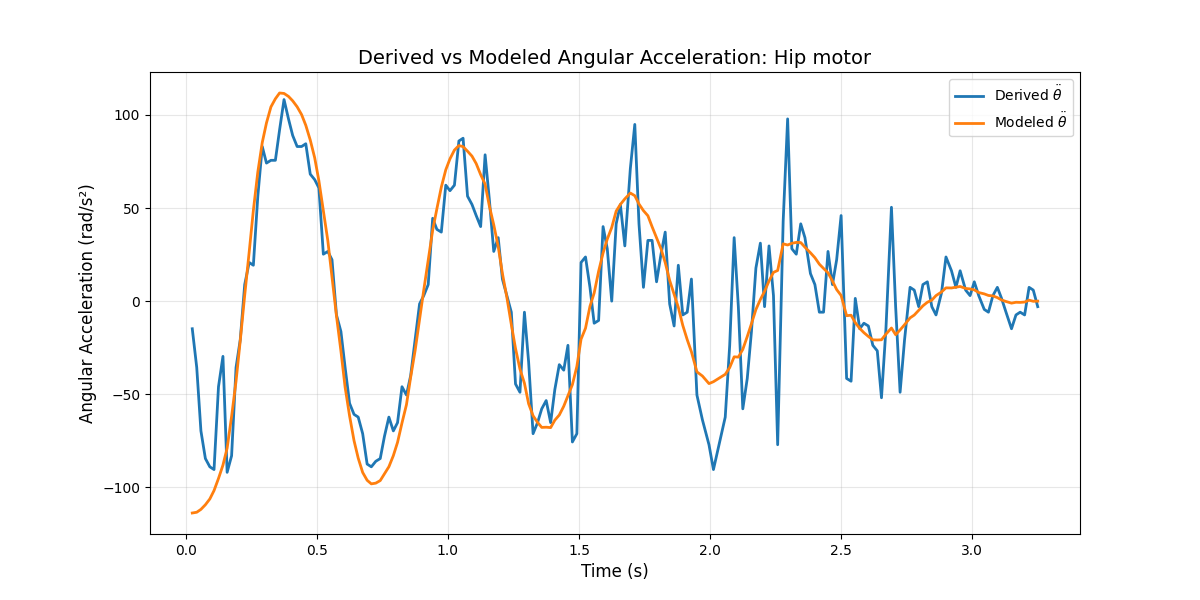
\includegraphics[width=0.8\textwidth]{Images/results/friction_est_hip_motor.png}
    \caption{Linear regression fit of the pendulum data for the hip motor.}
    \label{fig:results:motor_friction_estimation:linear_regression_hip_motor}
\end{figure}




\subsection{Link Length Optimization}
The grid search results for both Earth and Mars gravity are shown in figures \ref{fig:results:grid_search_earth} and \ref{fig:results:grid_search_mars}. The search explored link length ratios from 0.8 to 1.6 and total lengths from 8cm to 36cm, in increments of 0.1 and 0.5 cm respectively.

Best performing jumps are described in table \ref{tab:results:grid_search_earth:best_jumps}.
\begin{table}[h]
    \centering
    \begin{tabular}{lrrrrr}
        \hline
        Gravity & Jump Height (cm) & Ratio & Total Length (cm) & L1 (cm) & L2 (cm) \\
        \hline
        Earth & 118.03 & 1.0 & 35 & 12.5 & 12.5 \\
        Mars & 31.39 & 1.0 & 27 & 13.5 & 13.5 \\
        \hline
    \end{tabular}
    \caption{Best performing link length configurations and their corresponding jump heights for Earth and Mars gravity.}
    \label{tab:results:grid_search_earth:best_jumps}
\end{table}


\begin{figure}[h]
    \centering
    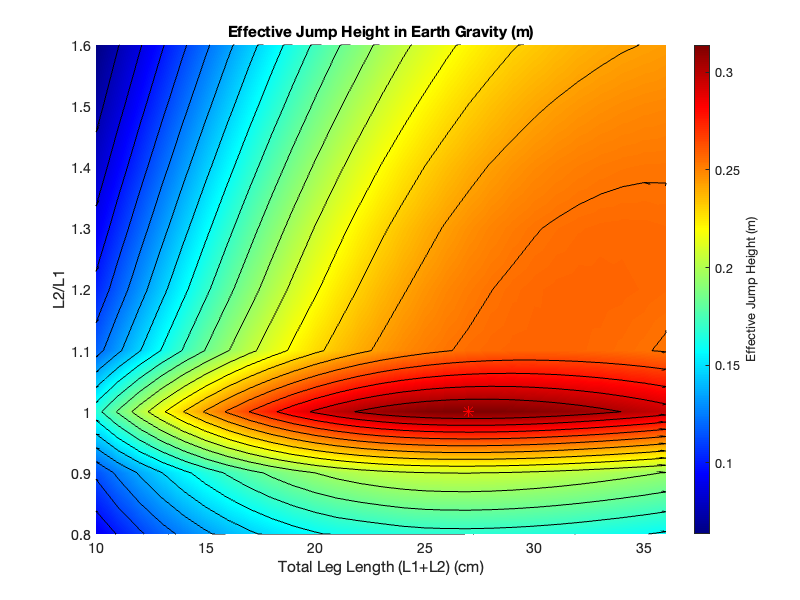
\includegraphics[width=0.8\textwidth]{Images/results/grid_search_results_earth_flat.png}
    \caption{Grid search results showing jump height performance across different link length configurations under Earth gravity.}
    \label{fig:results:grid_search_earth}
\end{figure}



\begin{figure}[h]
    \centering
    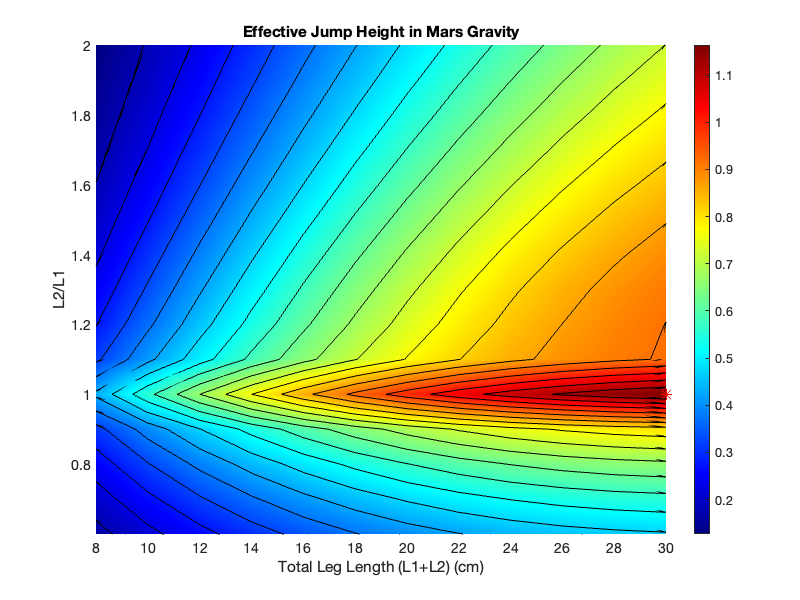
\includegraphics[width=0.8\textwidth]{Images/results/grid_search_results_mars_flat.png}
    \caption{Grid search results showing jump height performance across different link length configurations under Mars gravity.}
    \label{fig:results:grid_search_mars}
\end{figure}

TODO: Correct optima
The optimum total length is 8cm longer under Mars gravity. In both Mars and Earth gravity, the optimal link length ratio is 1.0 across all total lengths, with steep drops in jump height for ratios under 1.0 and less steep drops for ratios over 1.0. 

\subsection{Hip Motor Dimensioning Test}
\label{sec:hip_motor_dimensioning_test}

As can be seen in figure \ref{fig:hip_motor_strength_test}, the hip motors follow the angle reference well, achieving three back and forth swings of 90 degrees over a one second period. The torque output of the motors during this maneuver can be seen in figure \ref{fig:hip_motor_torque_test}. 

\begin{figure}[H]
    \centering
    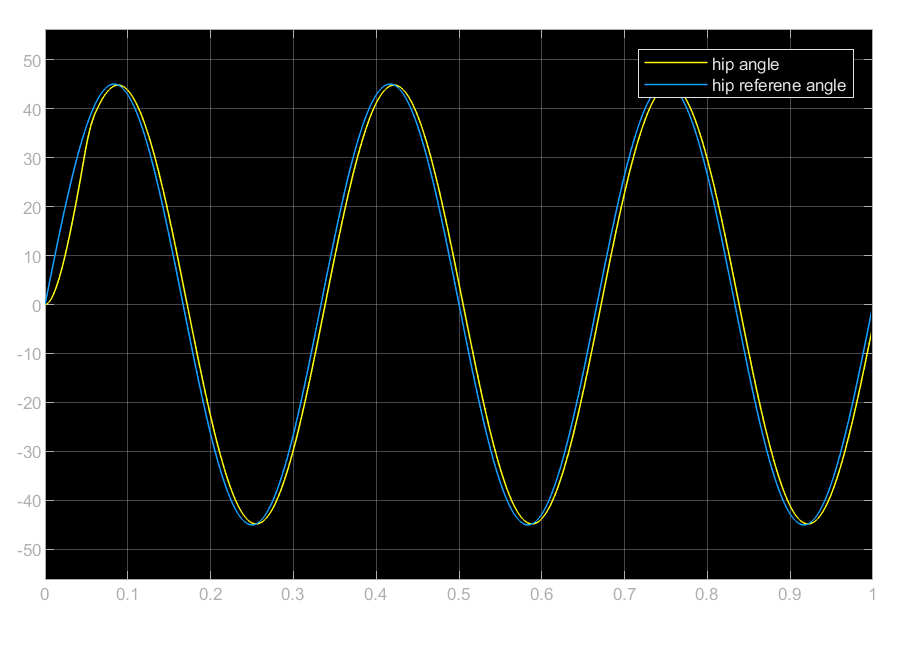
\includegraphics[width=0.8\textwidth]{Images/attitude_stable_test_result.eps}
    \caption{Commanded and actual hip joint angle achieved during the hip motor strength test simulation. }
    \label{fig:hip_motor_strength_test}
\end{figure}

figure \ref{fig:hip_motor_torque_test}.

\begin{figure}[H]
    \centering
    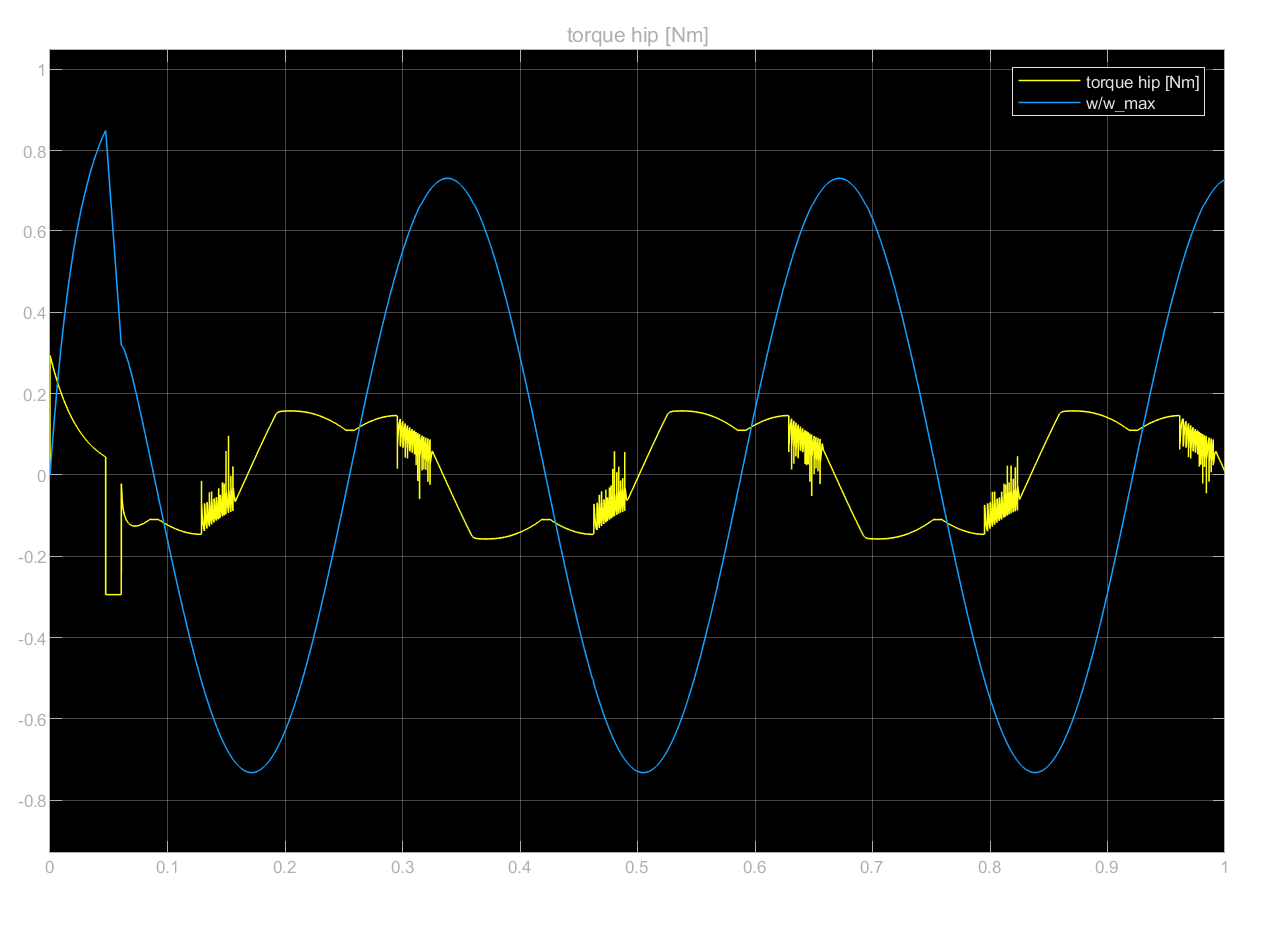
\includegraphics[width=0.8\textwidth]{Images/hip_motor_torque.eps}
    \caption{Torque output of the hip motors during the hip motor strength test simulation.}
    \label{fig:hip_motor_torque_test}
\end{figure}